\documentclass[showpacs,twocolumn,aps,floatfix,superscriptaddress,noshowpacs]{revtex4}
\usepackage[mathlines]{lineno}% Enable numbering of text and display math

\usepackage{amsthm,amsmath,amssymb,graphicx,bm,color,mathrsfs,verbatim,epstopdf,dcolumn,dsfont,cancel}
\usepackage{ulem,cancel,comment}

\usepackage{graphicx}


%define path for figs
\graphicspath{{figs/},
		  }

\usepackage{hyperref}
\hypersetup{ 
	colorlinks   = true
}

% Use following commands if you want to see comments and deletions
\newcommand*{\red}{\textcolor{red}}
\newcommand*{\blue}{\textcolor{blue}}
\newcommand*{\green}{\textcolor{green}}
\newcommand*{\pink}{\textcolor{pink}}
\newcommand*{\cyan}{\textcolor{cyan}}

% user-defined commands come here
\newcommand{\ra}{$\rightarrow$}

\DeclareMathOperator*{\argmin}{arg\,min}
\DeclareMathOperator*{\argmax}{arg\,max}

\begin{document}
	


%\preprint{APS/123-QED}

%\title{The quantum state preparation problem is equivalent to a glass !}% 
\title{Visualizing the clustering transition using unsupervised learning}%
%\title{The Spin Glass-like Phase of Optimal Quantum Control}%

\author{Alexandre G.R. Day}
\email{agrday@bu.edu}
\affiliation{Department of Physics, Boston University, 590 Commonwealth Ave., Boston, MA 02215, USA}

\begin{abstract}
We study the solutions of two random boolean satisfiability problems 3-SAT and XORSAT using recently developed machine learning techniques. We use non-linear embedding techniques to learn the local manifolds in which the solutions organize. In particular we provide, to the best of our knowledge, the first visualizing of the so-called clustering transitions that are known to occur in those problems. Finally, using unsupervised clustering methods we are able to automatically extract quantities such as the entropy of clusters.
\end{abstract} 

\date{\today}
%\keywords{Suggested keywords}
%\pacs{67.85.Pq, 71.10.Fd} 
\maketitle

Landscape induces complexity, but not always : \cite{ricci2010being}

\section{Introduction}
Chris Moore discussion, etc. cite M�zard, stat. phys. and yourself.

\begin{figure}[t!]	
	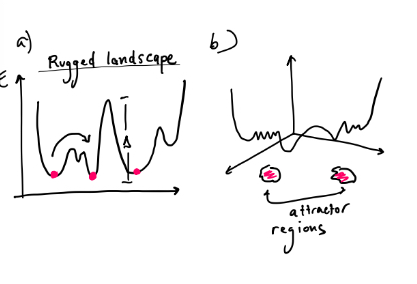
\includegraphics[width=1.0\columnwidth]{figs/fig1.png}
	\caption{\label{fig:schematic} Problem setting. (a) Rugged landscape cartoon picture. (b) In 3 dimensions we project attractors to a 2D space}
\end{figure}

\section{Model studied}
XORSAT, 3-SAT. 

\subsection{Method used}
BP, SP and Gaussian elimination.
\section{Results}

\begin{figure}[t!]	
	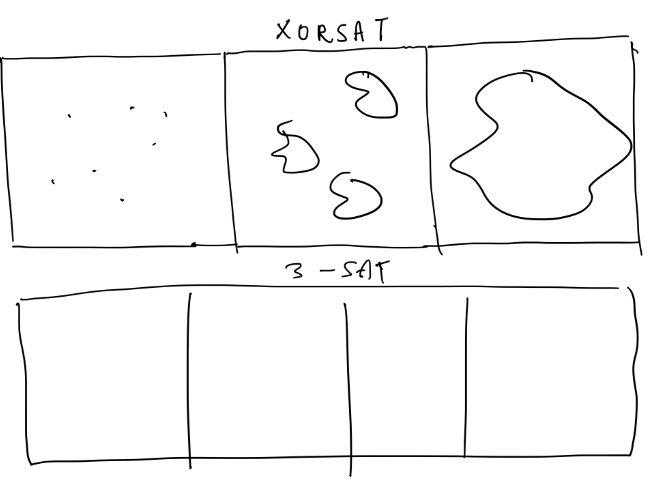
\includegraphics[width=1.0\columnwidth]{figs/fig2.png}
	\caption{\label{fig:tSNE} t-SNE visualization of the solution space as a function of the constraint parameter $\alpha$.}
\end{figure}


\begin{figure}[t!]	
	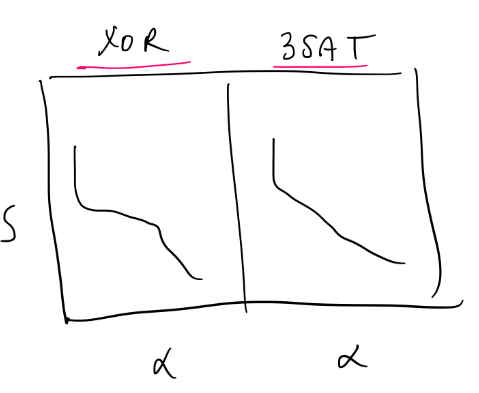
\includegraphics[width=1.0\columnwidth]{figs/fig3.png}
	\caption{\label{fig:tSNE} Entropy of clusters vs. $\alpha$.}
\end{figure}

\begin{figure}[t!]	
	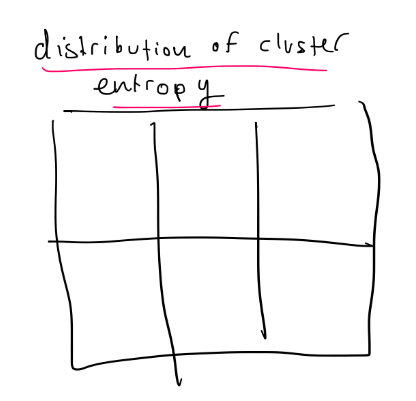
\includegraphics[width=1.0\columnwidth]{figs/fig4.png}
	\caption{\label{fig:tSNE} Distribution of cluster entropies at different $\alpha$.}
\end{figure}
\subsection{Density clustering}

\subsection{Results and Discussion}
Spin glass models such as the Sherrington-Kirkpatrick model or the Anderson model are known to be NP-complete \cite{venturelli2015quantum}. Consequently it is believed that no algorithm can be devised in order to compute the ground-state in a time scaling polynomially with the system's size. Much work has been made in trying understanding what makes a problem hard from a statistical mechanics point of view. In particular, in random satisfiability problems such $k$-SAT and XORSAT the onset of a glass transition has been associated with the appearance of frozen variables and clustering in the solution space, which has been conjectured to induce failure of local search algorithms \cite{moore2011nature}. Note that glassiness does not necessarily imply hardness to solve. Phenomenologically, it appears that for glassy problems, any local search/stochastic method will fail, i.e. finding the ground-state is exponential in the system size. However, if one is able to devise some global method based on non-local updates, then some glassy problems are known to be in $P$. This is the case for instance of XORSAT (equivalent to solving a linear system mod 2) which can be efficiently solved using gaussian eliminination \cite{ricci2010being}.
\paragraph{Clustering XORSAT, 3-SAT}
\paragraph{Entropy via density clustering}
Relation to complexity and broader applications in stat. mechanics.


\section{Conclusion}

Packages are available for t-SNE and efficient clustering available at alexandreday github

\section{Acknowledgements}


%State preparation plays a quintessential role in present-day studies of quantum physics. The ability to reliably manipulate and control quantum states has proven crucial to many physical systems, from the quantum mechanical emulators ultracold atoms~\cite{bason_12,vanfrank_16,wigley_16} and trapped ions~\cite{islam_11,senko_15,jurcevic_14}, through solid-state systems like superconducting qubits~\cite{barends_16}, to nitrogen vacancy centres~\cite{zhou_17}. The non-equilibrium character of quantum state manipulation makes it a difficult and not well-understood problem of ever increasing importance to building a large-scale quantum computer~\cite{nielsen}.
%
%Analytically, state preparation has been studied using both Adiabatic Perturbation Theory~\cite{kolodrubetz_16} and Shortcuts to Adiabaticity~\cite{demirplak_03,delcampo_13,jarzynski_13,sels_16}. Unfortunately, these theories have limited application in non-integrable many-body systems, for which no exact closed-form expressions can be obtained. This motivates the development of efficient numerical algorithms, such as GRAPE~\cite{glaser_98, grape_05}, CRAB~\cite{caneva_11}, and Machine Learning~\cite{judson_92,chen_14,chen_14_ML,bukov_17RL,yang_17,dunjko_17,august_18,foesel_18,sorensen_18,zhang2018automatic}. The objective in Optimal Control theory is to find the set of controls that extremize a cost function, e.g.~ determine the optimal fidelity to prepare a target state, subject to physical and dynamical constraints. However, cost functions, usually defined on a high-dimensional space, are typically non-convex, and therefore there exist no algorithm guaranteed to find the optimal (global) solution in \emph{general}. Moreover, optimality does not automatically imply stability and robustness of the solution, which are required for experimental applications. Establishing the general limitations and constraints of quantum control is crucial for guiding the field forward.
%%Therefore, a fresh perspective on this old conundrum would be appreciated.  ?? ok maybe more enthusiasm here !
%\begin{figure}[t!]	
%	\includegraphics[width=1.0\columnwidth]{figs/schematic.png}
%	\caption{\label{fig:schematic} Problem setting. (a) A nonintegrable 1D Ising model subject to a global control transverse field $h(t)$. We focus on the family of bang-bang protocols with $h(t)$ taking values $\pm 4$. (b) Every bang-bang protocol generates an evolution from an initial to a final state from which we compute a fidelity w.r.t. the target state. For a discretization with $N_T$ time steps, there are $2^N_T$ bang-bang protocols. The set of fidelities associated to the bang-bang protocols defines a spectrum. (c) Schematic representation of a rugged fidelity landscape. (d) Moving from one protocol to another requires ``flipping" the signs of $h(t)$ at different times. }
%\end{figure}

%\emph{Model studied and methods.---}Consider quantum spin-$1/2$ degrees of freedom $S^\mu_j$ described by the Ising model with a time-dependent transverse-field (c.f. Fig \ref{fig:schematic}.a): % defined by the Hamiltonian
%\begin{equation}
%\label{eq:H}
%H(t) = -\sum_j JS^z_{j+1}S^z_j + g S^z_j + h(t)S^x_j,
%\end{equation}
%with interaction strength $J\!=\!1$ (sets the energy scale), and an external magnetic field of a static $z$-component $g\!=\!1$ and a bounded time-varying $x$-component $\vert h(t)\vert\!\leq\! 4$. The presence of the longitudinal $z$-field renders the model non-integrable at any fixed time $t$, with no known closed-form expression for the exact instantaneous eigenstates and eigenenergies. We work in a non-perturbative regime with all couplings of similar magnitude. 

\emph{Acknowlegements.---}


%We thank ... for illuminating discussions. AD was support by an NSERC PGS-D. AD and PM acknowledge support from Simon's Foundation through the MMLS Fellow program. MB acknowledges support from the Emergent Phenomena in Quantum Systems initiative of the Gordon and Betty Moore Foundation and the ERC synergy grant UQUAM. DS acknowledges support of the FWO as post-doctoral fellow of the Research Foundation - Flanders. We used \href{https://github.com/weinbe58/QuSpin#quspin}{Quspin} for simulating the dynamics of the qubit systems~\cite{weinberg_17}. The authors are pleased to acknowledge that the computational work reported on in this paper was performed on the Shared Computing Cluster which is administered by \href{https://www.bu.edu/tech/support/research/}{Boston University's Research Computing Services}. The authors also acknowledge the Research Computing Services group for providing consulting support which has contributed to the results reported within this paper.

\bibliographystyle{apsrev4-1}
\bibliography{ref}

\newpage

\begin{widetext}

\section*{\large Supplemental Material}


\section{\label{sec:densecluster} Density clustering via kernel density estimates}

\end{widetext}
\end{document}